\documentclass{llncs}

\usepackage{subfigure,epsfig,wrapfig}
\usepackage{makeidx} % allows for indexgeneration
\usepackage{epsfig,wrapfig}
\usepackage{amsmath,amscd,stmaryrd,graphicx,caption}
\usepackage{amssymb,amsmath,latexsym}
\usepackage{subfigure,wrapfig}
\usepackage{listings}
\usepackage{float}
\usepackage{color}
\usepackage{multirow}

\input xy
\xyoption{all} % Reference for references: http://www.brics.dk/~krisrose/Xy-pic.html

\newtheorem{defi}{Def.}
\newtheorem{prop}{Prop.}
\newcommand{\abb}[3]{#1 \colon #2 \rightarrow #3}

\newcommand{\cosp}[5]{#1 \overset{#4}\rightarrow #2 \overset{#5}\leftarrow #3}
\newcommand{\dporule}[5]{#1 \overset{#4}\leftarrow #2 \overset{#5}\rightarrow #3}
\newcommand{\longdporule}[5]{#1 \overset{#4}\longleftarrow #2 \overset{#5}\longrightarrow #3}

\newfloat{model}{thp}{lop}
\floatname{model}{{\bf Listing}}

\newcommand{\figepsr}[4]{ % {FIGNAME}{FACTOR}{ANGLE}{CAPTION} }
   \begin{figure}[h!tb]
       \def\epsfsize##1##2{#2##1}
       \centerline{\rotatebox{#3}{\epsfbox{figures/#1.eps}}}
       \caption{#4}
       \label{fig:#1}
    \end{figure}
}

\newcommand{\figeps}[3]{ % {FIGNAME}{FACTOR}{CAPTION} }
    \begin{figure}[t]
        \def\epsfsize##1##2{#2##1}%
        \centerline{\epsfbox{figures/#1.eps}}
        \caption{#3}
        \label{fig:#1}
     \end{figure}
}

\begin{document}

\pagestyle{headings} % switches on printing of running heads
%\addtocmark{XXXX} % additional mark in the TOC

\title{Umbra Designer: Graphical Modelling for Telephony Services} % title
\titlerunning{Bender} % abbreviated title (for running head) also used for the TOC unless \toctitle is used

\author{Nicol\'as Buezas\inst{1} \and Esther Guerra\inst{1} \and Juan de Lara\inst{1} \and Javier Mart\'in\inst{2} \and Miguel Monforte\inst{2} \and Fiorella Mori\inst{1} \and Eva Ogallar\inst{2} \and Oscar P\'erez\inst{2} \and Jes\'us S\'anchez Cuadrado\inst{1}}
\authorrunning{Buezas et al.} % abbreviated author list (for running head)

%%%% modified list of authors for the TOC (add the affiliations)
\tocauthor{
Juan de Lara (Universidad Aut\'onoma de Madrid),
Esther Guerra (Universidad Aut\'onoma de Madrid),
Jes\'us S\'anchez Cuadrado (Universidad Aut\'onoma de Madrid)
}

\institute{
Department of Computer Science\\
Universidad Aut\'onoma de Madrid (Spain)
\and
Almira Labs, S. L.\\
Science Park -- Tres Cantos, Madrid (Spain)\\
\url{http://www.almiralabs.com}
%\email{\{Juan.deLara,Esther.Guerra\}@uam.es}
}

\maketitle

\begin{abstract}
Almira Labs is a software company that develops value-added services for the telecommunications industry.
It is focused on innovative technologies that enable enterprise business and mobile and landline operators
to offer next-generation voice-driven applications for all types of phones. Telephony services are built atop 
the proprietary {\em Umbra framework}, which is a Java API relying on the JAIN SLEE standard for event-based 
communication applications.

This paper describes {\em Umbra Designer}, a novel graphical modelling tool for the visual development of 
telephony services, from which Java code for the {\em Umbra framework} is synthesized. In this way, it is easy
to develop ready-to-use services, even by users not familiar with the Java API or the JAIN SLEE standard. We also 
report on some experiments aimed at measuring the efficiency gain derived from using the graphical tool, compared
with coding directly using the Java API.
\end{abstract}

\begin{keywords} 
Model-Driven Engineering, 
Telephony Services, 
Jain SLEE, 
Domain Specific Visual Languages, 
Code Generation\end{keywords}

\section{Introduction}\label{sec:introduction}
We are witnessing an exponential grow in the capabilities of mobile phones and in the functionality demanded by 
their users. The usual approach to deliver mobile services nowadays is the development of {\em apps} 
for a particular technology (iOS, Android, BlackBerry), running in the device of the client. This business model is 
supported by small software firms that need to develop innovative solutions in short times, in order to cope with 
an increasingly competing environment. This model has the drawback of the fragmentation of the mobile platforms, 
which implies different developments for each platform. Moreover, the functionality offered by different phones varies, 
from traditional landline phones to smartphones of the latest technology. Thus, companies may lose clients if they 
target particular platforms or assume some functionality for running their {\em app}~\cite{5640901}. 

Instead, a different alternative is to build services that do not run on the phone, but on the provider infrastructure
through dedicated servers or the cloud, and which are accessed through phone calls~\cite{Almira}. This model has the 
advantage that is independent of the mobile phone platform used, and to a certain extent, of the phone capacities. While 
these ``server-side'' services cannot replace all types of phone {\em apps}, they are useful for many scenarios. They
are normally driven by voice and DTMF key strokes. Examples include voice notes and voice-to-email services; 
services to inject customized background sounds in phone calls; the customization of the telephone keys to inject 
``voice smileys'' in a conversation; as well as the typical Interactive Voice Response (IVR) applications of call 
centers, telebanking, credit card services, and so on. These services tend to require a reduced customer learning curve
compared to those offered by mobile {\em apps}.

JAIN SLEE~\cite{JAINSLEE} is a standard of the Java Community Process for developing event-based 
telecommunication applications, which can be used to build server-side telephony services. Applications 
developed with JAIN SLEE can be deployed on any server implementing it. A Service Logic Execution 
Environment (SLEE) is an efficient event processing application environment with high throughput and 
low latency. A service is built by the construction and interconnection of components, and their subsequent
deployment in SLEE servers.

Almira Labs has developed the {\em Umbra framework}, a Java API that leverages 
on the JAIN SLEE standard. The framework simplifies the development of JAIN SLEE applications by providing 
a higher-level view of the event flows and protocols involved in a telecommunications application, and provides 
true portability across different SLEE implementations. 
Still, using this framework requires specialized knowledge in JAIN SLEE and Java. In order to make service 
construction possible for non-experts -- namely, people from customer companies -- Almira and some 
researchers of the Universidad Aut\'onoma have developed {\em Umbra Designer}, a tool for the graphical
development of telephony services. The tool abstracts services in the form of hierarchical state machines using the 
events and actions available in the {\em Umbra framework}. 
The tool integrates a code generator that produces a {\em Maven}~\cite{Maven} Java project, which 
can be deployed as-is in JAIN SLEE servers for execution. The aim of the tool is to facilitate 
service modelling to non-experts in the API, and speed-up the development for programmers. This is 
demonstrated by a series of experiments where we have measured the efficiency of manual service 
development using the Java API with respect to using the tool, reporting an increase of productivity of 
more than 40\% in the average case.

\paragraph{Paper organization.} Section~\ref{sec:api} provides some background on 
JAIN SLEE and the {\em Umbra framework}. Section~\ref{sec:designer} introduces the graphical 
modelling tool. Section~\ref{sec:evaluation} presents the evaluation results. Section~\ref{sec:related} 
compares with related work, and finally, Section~\ref{sec:conclusions} ends with the conclusions and plans 
for future work.


\section{Programming voice-driven telephony services}\label{sec:api}
Our work targets at voice and key-strokes driven telephony services. These services normally run on the
infrastructure of the service provider. Subsection~\ref{sec:JSLEE} reviews a standard (JAIN SLEE) that can be used for building
this kind of applications, while subsection~\ref{sec:umbra-framework} introduces a Java framework built atop JAIN SLEE
which provides higher-level abstractions and true portability across SLEE implementations.

%---------------------------------------------------------
\subsection{JAIN SLEE}\label{sec:JSLEE}
%---------------------------------------------------------

JAIN SLEE is a standard by the Java Community Process that describes
a Service Logic and Execution Environment (SLEE) architecture~\cite{JAINSLEE}.
This architecture defines a component model for structuring the logic of communications applications
as a collection of object-oriented components (called Service Building Blocks, SBBs), which can be composed into
services. The SLEE architecture also defines the contract between these components
and the container that will host them at runtime. 
JAIN SLEE applications are event-driven, which means that methods of the application are invoked when
suitable events arrive. In this way, each SBB to be deployed in the SLEE identifies the event types 
that accepts, and defines event handler methods with code to process such event types. 

The framework provides an API for handling events, resources and connections, facilities like timers 
and alarms, and standard interfaces to be implemented by SBBs. Still, the API is low-level, and 
service developers would benefit from higher-level abstractions, tailored to voice-driven telephony 
services, as explained in the next subsection.

%-------------------------------------------------------------------------------
\subsection{The Umbra Framework}\label{sec:umbra-framework}
%-------------------------------------------------------------------------------

The {\em Umbra framework} hides the low-level details of JAIN SLEE to enhance performance and simplify 
the development of telephony services. It masks the JAIN SLEE components behind a simpler Java API that offers 
enhanced, scalable, carrier-grade performance. Another benefit is portability. As different providers offer 
different implementations of the standard, there may be JAIN SLEE compliant applications that do not run 
on every SLEE container. Moreover, when migrating an application from one vendor to another, parts
of its code may need to be re-written to ensure smooth porting and compatibility. With the {\em Umbra 
framework}, the code works across JAIN SLEE platforms from the main vendors without any recoding.

The framework enables building applications mixing both web and telephony services.
While JAIN SLEE can deal with low-level protocol issues at the back-end, a J2EE environment can provide a 
front-end for Internet services. Hence, {\em Umbra} enables the SLEE to offer web services the J2EE world can interact with.
%so that the J2EE world can interact with the network capabilities exposed by the SLEE.

Fig.~\ref{fig:UmbraStructure} shows the typical structure of a service built with the {\em Umbra framework}. 
The upper part shows only the most relevant interfaces provided by the framework. The lower part (package 
{\em application}) presents a schema of the classes and interfaces that programmers have to develop. 
As we will see, {\em Umbra} is based on the definition of suitable event types and listeners for such events. The
listeners contain call-back methods, invoked upon the reception of the events, which need to be programmed
by the service developers.

\figeps{UmbraStructure}{0.42}{Structure of an application using the {\em Umbra framework} (simplified).}

A service is started upon the reception of the {\em onBootstrap} event. Hence, the developer needs to 
implement code to react to this event in the {\em BootStrapEventListener}. Normally, 
this code includes loading the needed resources and register event listeners  
through a {\em ServiceLocator}, especially {\em SessionRequest} events, which are events triggered by 
the SLEE container when the network requests a new session. Then, the service waits for incoming events, which
may trigger specific actions like playing a message, recording a message, soliciting the user to press a key,  
and so on. These actions are supported by an {\em IVRServer} (a media server), which is a resource
that needs to be identified upon bootstrap. The service will receive an event notification upon completion of the 
actions, as declared in the {\em IvrServerEventListener}. For example, the {\em onPlayed} method will be 
called upon completion of a {\em play} action, which plays a voice message.

Practice has shown that a suitable organization for event-driven applications is through state machines.
Hence, a typical programming idiom for services built with the {\em Umbra} framework is the {\em State 
pattern}~\cite{Gamma} in order to describe the different execution states of the service, the possible 
incoming events, the actions to be performed upon the arrival of events, and the state changes. This way,
services normally define an interface {\em State} declaring all possible events, while the abstract class 
{\em AbstractState} defines default empty implementations for the event handlers. Therefore, developers 
have to create a subclass of {\em AbstractState} per application state ({\em State1} in Fig.~\ref{fig:UmbraStructure}), 
and override the methods for the events accepted by the state.

This organization is a Java implementation of a natural way of designing services as state machines. 
However, this style of programming is not enforced by the {\em Umbra framework}
even though it is common practice. Hence, we decided to provide developers with a higher level representation of this pattern, closer
to the abstractions of state machines. This way, the gap from design to implementation would be smaller. 
Moreover, this representation would facilitate the communication with customers, most frequently
non-technical people. The next section introduces a Domain-Specific Visual Language that helps in describing 
services at a higher level of abstraction.




\section{Modelling telephony services with Umbra Designer}\label{sec:designer}
Fig.~\ref{fig:schema} shows the architecture of our solution. The developer or designer graphically defines
the services using {\em Umbra Designer}. We have built this tool as an Eclipse plugin, using Graphiti~\cite{Graphiti} 
for the visual part, EMF~\cite{EMF} as modelling technology, and the Epsilon Generation Language (EGL)~\cite{EGL} 
for code generation. After validating the service, the tool generates a Maven project with code synthesized from
the service. The code makes use of the {\em Umbra framework}, as explained in the previous section. Once compiled, 
the project can be deployed as-is on SLEE servers, like the {\em open cloud}'s Rhino application server~\cite{rhino}.

\figeps{schema}{0.48}{Schema of {\em Umbra Designer}.}

Next, we introduce the main elements of the tool. Fig.~\ref{fig:servicio1} shows a screenshot with an example service. 
The tool abstracts services in the form of state machines, accommodating the State design pattern, as explained above.

The main canvas contains the description of a simple service. The service initial state is {\em Init}, where the 
service waits for incoming calls once a new session has been established. Hence, at the top level, the event from the 
initial state is {\em SessionRequest} (see arrow coming into state {\em Init}). The service designer does not 
have to take care of handling the {\em Bootstrap} event, as the tool itself will generate code to register the 
listeners for the events and actions used by the service (in the example all are {\em IVR} events), and identifying 
the needed resources. Events are depicted in blue (bold) over the arrows, while actions are shown in red below 
the events. The service plays a welcome message to each incoming call. This is modelled by a {\em Connected} 
event and the associated {\em PlayCollect} action. This action has the additional effect to demand pressing 
some key on the phone keypad. Thus, the service waits in state {\em KeyRequest} until the reception of some key 
stroke (event {\em Collected}). If the key pressed was ``1'' or ``2'', the service plays a different message 
in each case, as indicated by the {\em Play} action. Once the message associated to ``1'' or ``2'' is played 
(event {\em Played} in the transition going out from {\em Bye}), the service ends the call through the {\em Hangup} 
action.

\figeps{servicio1}{0.3}{Defining a simple service with {\em Umbra Designer}. }

The palette to the right contains the different types of states, transitions (i.e. events) and actions that can
appear in services. The Properties view at the bottom allows configuring any item selected in the model; in the
figure, it shows the configuration properties of the service and its resources. The tool has a contextual menu 
to validate the service (the detected warnings and errors are listed in the Problems view at the bottom), to 
generate Java code from the service, and to manage the generated Maven project (the project is shown in the 
Project Explorer tab to the left). 

Altogether, the tool promotes an agile way to work, providing support for short cycles of modelling -- 
code (re-)generation -- deployment in an integrated environment. For instance, once code is generated
for a service, developers can provide additional Java classes for further functionality 
(e.g. database persistence, which is not currently supported by our tool). We believe that this approach to 
agile modelling will be better accepted in development processes as it provides immediate value by code 
generation and service validation, and it is seamlessly integrated in the developer Java environment.

The abstract syntax of the services built with our tool is defined through a meta-model, of which
Fig.~\ref{fig:UmbraDesignerMetaModel} shows an excerpt. A state machine is configured through a 
number of properties (class {\em Properties}), like the addresses of the application and server, and 
the protocols used, among others. It is also possible to declare variables that will be available in
Java actions. Two different types of variables are supported: shared variables (object attributes), 
used to pass information between different service states, and static variables (class attributes), 
which retain their value between different service invocations. 

\figeps{UmbraDesignerMetaModel}{0.5}{Excerpt of the {\em Umbra Designer} meta-model.}

We consider five types of states: initial, final, simple, composite and choice. Each state machine has 
one initial and one final states. Composite states enable hierarchical structuring of the machine, and 
contain a reference to a state machine which can be defined within the same model or externally in a 
separate file. Choice states have multiple output branches with a boolean condition each.

Transitions can be of different types that correspond to event types of the {\em Umbra framework}. 
They are organized in six categories: Interactive Voice Response (IVR) events, Call Control events, 
HTTP (reception of HTTP requests), SMS, Text-to-Speech (TTS) and Speech recognitions events 
(for clarity, Fig.~\ref{fig:UmbraDesignerMetaModel} only shows IVR events). There are also general 
facilities, like timers. The initial event in a state machine is always of type {\em SessionRequest}.
IVR events are concerned with playing and recording media streams or with key pressing in the phone keypad. 
Examples of supported IVR events include {\em Played} (fired when a media stream finishes playing), 
{\em Recorded} (when a recording finishes) and {\em Collected} (when the user presses some key). 
Call control events include those related to the connection, disconnection and transfer of call legs. SMS 
events are concerned with the reception of text messages. Finally, TTS events are those generated by 
a TTS engine, like the start, finish, pause and resume of a speech.

A transition may have associated a sequence of actions, to be executed when the transition is triggered. 
Actions rely on the {\em Umbra} API, and are organized in similar categories to those for events. A 
special action {\em JavaCode} permits adding Java code for more general actions not directly supported 
by the framework, where it is possible to use the declared shared and static variables. The parameters 
of each action can be configured through a properties panel, as shown to the bottom of Fig.~\ref{fig:repairingService} 
for the case of the {\em PlayRecord} action.

{\em Umbra Designer} supports hierarchical modelling by means of composite states (see {\em MembersMenu}
in Fig.~\ref{fig:hierarchy}), and through references to state machines defined in other diagrams (see state 
{\em Registration} in the same figure). In the last case, a contextual menu allows opening the referenced 
machine in a different tab, as well as expanding or occluding the diagram inside the state. This feature enables
the construction of repositories of services, which then can be used to build other more complex services.

\figeps{hierarchy}{0.3}{Hierarchical modelling, and report of errors/warnings, in {\em Umbra Designer}.}

The tool enables simple validations of services prior to code generation, and displays the detected errors 
and warnings in the Eclipse Problems view (see bottom panel in Fig.~\ref{fig:hierarchy}, which contains
the detected list of errors for an information and registration service for a gym). For example, the tool reports
as an error any unreachable state, any state (different from the final state) without outgoing transitions, as well 
as non-existing paths between the initial and final states. Warnings concern the order in which some events and 
actions should occur, as some actions trigger the future occurrence of events. For example, the tool gives a 
warning if a {\em Played} event is declared, but there is no previous {\em Play} action. Notice that all these 
errors and warnings would be difficult to detect statically, if a direct encoding of the service in Java is used. 
However, we do not currently analyse {\em JavaCode} actions in transitions.

Once the model of the service is validated, it is possible to synthesize Java code from it. The tool creates a Maven 
Eclipse project, which can be deployed in an SLEE server. The generated Java code follows the State pattern~\cite{Gamma}, 
and reflects the hierarchical constructs introduced in the model. Moreover, the code includes protected regions, 
so that if the developer modifies the code manually, this is not overwritten when code is regenerated again from 
the model. 


\section{Evaluation}\label{sec:evaluation}
In order to asses to what extent using {\em Umbra Designer} improves the productivity of service development,
we have performed an experiment consisting in the construction of ten services of varying complexity using the 
graphical tool, and the comparison with the effort to develop the same services using directly the framework API
(i.e. programming directly in Java). 

We had two participants in our experiment, both last year undergraduates in Computer Science. The first
participant had some knowledge of telecommunications services, but no deep knowledge of the {\em Umbra 
framework}'s API. The second participant had some 5 months of experience using the API. 
Each participant built 5 services using the tool and 5 different ones using the API.
Each service was built in a different session, on a different day. The participants were given enough time
to read each service description and think a solution. When they were ready, we measured the time they
employed to implement the solution, one using the graphical tool and the other using directly the Java API. 
This way, we leave out effects related to problem understanding and solution design, and strictly measure
service production efficiency by two different means.

The services used in the experiment varied in complexity, ranging from simple ones (five states
%, including initial and final, 
and few transitions) to medium size (more than 15 states and 35 transitions). In each session, the participants 
were given textual definitions of the service to be developed in the session. As an example, the description of one 
of the services was the following: ``{\em Build a voice service for a computer repair shop. The service will play a 
message, and then, it will solicit the year in which the computer was bought. The user should type the solicited 
year using the telephone keyboard. Then, if the computer is still in the guarantee period (2 years), the service 
will solicit the serial number and the address, which will get recorded}''. 
Fig.~\ref{fig:repairingService} shows the service finally built for the previous service definition, 
using the graphical tool. The Properties view contains the configuration of the actions in the transition
entering state {\em SolicitarDireccion} ({\em Solicit Address}). The transition has two actions, one for recording
the address (whose configuration is shown), and the other one is just one line of Java code to transform the 
different key strokes into a String service variable (not shown).

\figeps{repairingService}{0.3}{Service \#7: a simple service for a computer shop.}

Other services built include a game for guessing a number, a time service which informs of the current time, 
a taxi call service, a simplified airport information service and a service for pizza ordering (see Table~\ref{tab:results}).

Table~\ref{tab:results} summarizes the experiment results. The columns show: (1) the name of the service;
(2--5) the size of its model-based solution (number of states and transitions, cyclomatic complexity and lines of extra 
Java code in {\em JavaCode} actions); (6--7) the number of source lines of code (SLOC, not 
counting blank lines or comments) of the service that are generated by the tool or hand-coded using the API; (8--9) 
the minutes taken to build the service using the tool and the API; and (10) the efficiency gain when using the tool 
compared to using the API (minutes and percentage). In the case of using the API, the measurements also include 
the creation time of additional artefacts, like property files, needed to deploy the service (but automatically generated by the tool).

\begin{table}[h]
\centering
\scriptsize
\begin{tabular}{|p{0.7cm}p{2.0cm}||p{0.9cm}|p{0.9cm}|p{0.9cm}|p{0.9cm}||p{0.8cm}|p{0.8cm}||p{0.8cm}|p{0.8cm}||p{1.5cm}|}
\hline
&        		& \multicolumn{4}{|c||}{{\bf Model Size}} & \multicolumn{2}{|c||}{{\bf SLOC}} & \multicolumn{2}{|c||}{{\bf Time (min.)}}  & \\ \hline
&        		& States & Trans.  & Cycles & Java Extra & Tool & API                                     & Tool & API                            & {\bf Gain (min./\%)} \\ \hline
\#1 : & Message + Key  & 5        & 6         & 3        & 0 & 383 & 395 & 7                    &  30            & {\bf 23 (76\%)} \\ \hline
\#2 : & Taxi Call           & 8        & 10       & 4        & 2 & 441 & 403 & 9                    &  21              & {\bf 12 (57\%)} \\ \hline
\#3 : & Guessing Game & 8        & 13       & 6        & 3 & 448 & 415 & 23                  &  42            & {\bf 19 (45\%)} \\ \hline
\#4 : & Postal Code/ Time Warning & 6        & 12       & 8        & 12 & 439 & 453 & 30 &  53          & {\bf 23 (43\%)} \\ \hline
\#5 : & Traffic              & 9      & 12         & 5      & 4 & 450 & 453 & 20                  &  35              &  {\bf 15  (42\%)} \\ \hline
\#6 : & Survey             & 10      & 14       & 6        & 0  & 529 & 477 & 15                  &  33            & {\bf 18 (54\%)} \\ \hline
\#7 : & Computer Shop & 9       & 13         & 6        & 4 & 493 & 501 & 20                  &  40             &  {\bf 20 (50\%)} \\ \hline
\#8 : & Airport             & 11      & 23         & 14      & 8 & 542 & 514 & 60                  &  90             & {\bf 30  (33\%)} \\ \hline
\#9 : & Time Service    & 5        & 4         & 1        & 269 & 640 & 749 & 24                  &  36             & {\bf 12 (33\%)} \\ \hline
\#10 : & Pizza Orders   & 17     & 52         & 37      & 60 & 963 & 925 & 150                &  200            & {\bf 50 (25\%)} \\ \hline
\end{tabular}
\caption{Evaluation of the construction of several services.}
\label{tab:results}
\end{table}
%\#7 : & Simple Message & 6                  &  15           & 7        & 10         & 5        & 2           & 16         & 949 \\ \hline

The experiments show good correlation between the number of SLOC of the hand-coded solution and of the code generated by the tool. 
Regarding productivity, by using the tool we observe an increase of around 45\% in the average case. In all cases, 
the time to develop a service with the tool
was less than using the API directly. Fig.~\ref{fig:graphics}(a) shows a graphic showing the net gain with respect to service size (SLOC
of the hand-coded solution), 
while the right shows the percentage gain with respect to size. The graphic shows higher percentual gains for smaller services; however, the highest net gain was with the 
largest service. We noted higher gains in cases were the service accommodated well the abstractions of state machines: few cycles, few decision
nodes, and few extra lines of code.

\begin{figure}[h!tb]
  \centering
    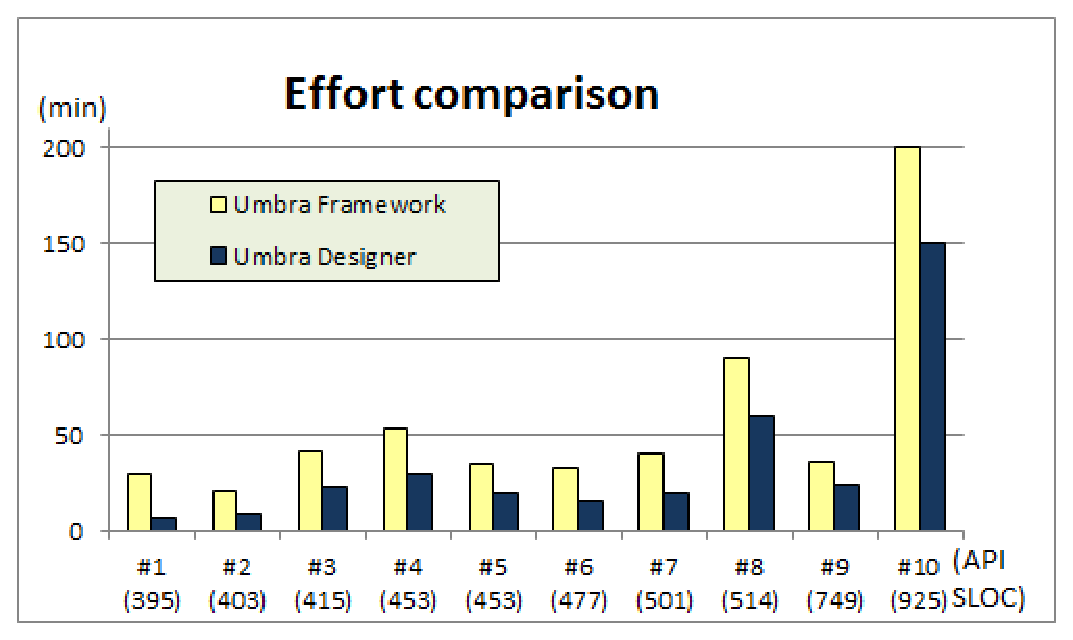
\includegraphics[scale = 0.35]{figures/effort.eps} %\caption{A figure \label{fig:figure}}
  \hspace{0.1cm}
    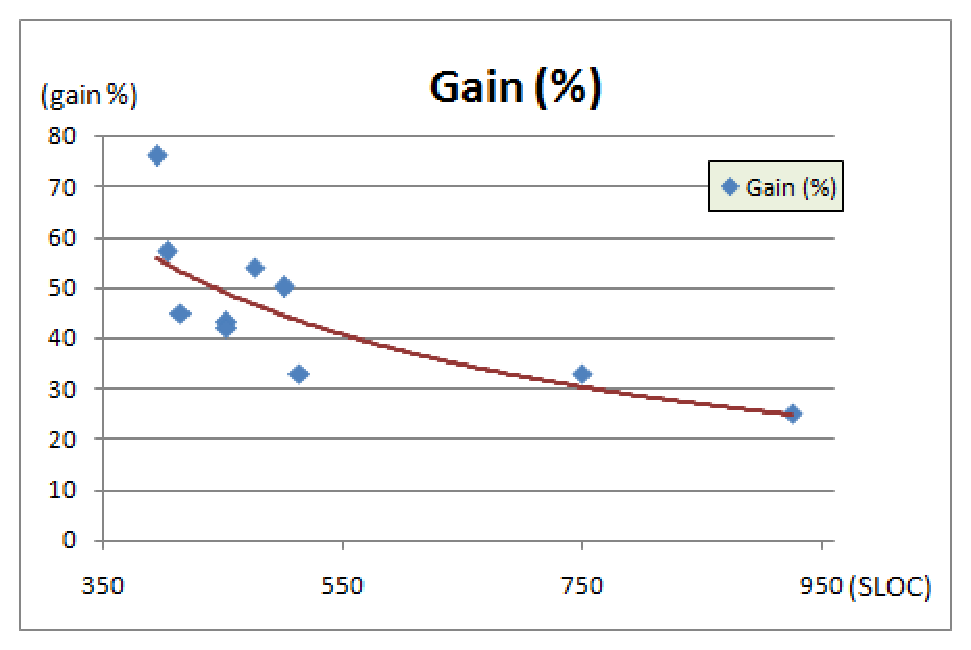
\includegraphics[scale = 0.35]{figures/gain.eps} %\caption{Another figure \label{fig:another}}
  \caption{Development effort comparison (left). Efficiency gain (right).}
  \label{fig:graphics}
\end{figure}

Altogether, the experiment shows benefits in efficiency when using the graphical tool. Moreover, we believe that it provides further benefits 
concerning: built-in validation checks, maintainability, understandability and reutilization of services. Experiments to assess these properties are 
subject to future work. As a preliminary result, we experienced in measuring the effort gain in maintainability, where a modification to service \#1 
consisting in the introduction of an error message on certain events was introduced. In this case, using the graphical tool led to shorter times 
(6 minutes vs 15 minutes). A finding related to this issue was that both participants found useful to draw state machine-like diagrams on paper, 
as a design sketch, before starting coding using the API. This means that the graphical model was deemed a good abstraction to describe services.

\section{Related work}\label{sec:related}
The need for developing and making available telecommunication APIs, is discussed in~\cite{5640901}. Similar to our rationale, the author
foresees the possibility of telecommunication application stores -- similar to those of Apple and Android -- based on the availability of service creation environments. 
%While most large companies offer different forms of service creation environments and deployment frameworks, they are closed systems. (?)

There are several implementations of the JAIN SLEE, like Mobicents~\cite{Mobicents} and
OpenCloud~\cite{rhino}. The latter includes a visual builder for services, the
Visual Service Architect (VSA)~\cite{VSA}. In this environment, a service is described by an application-scenario diagram (to configure properties, protocols and
resources), state machine diagrams (to describe service states) and flowchart diagrams (to describe actions). VSA targets general JAIN SLEE 
services, not necessary for telephony, and hence lacks high-level constructs (both events and actions) for voice-driven telephony services, as we 
provide in {\em Umbra Designer}. VSA state
machines and flowcharts tend to be of lower level of abstraction due to the lack of constructs like hierarchical states, choice states and key strokes
branches, among others.

In~\cite{ICT}, the authors present an environment for service composition using MetaEdit+. SBBs are programmed 
in Java, which become reusable and can be composed graphically. Our approach is different as the blocks themselves 
are modelled using state machines, from which Java code is generated. Also in the context of MetaEdit+, in~\cite{DSVLs}, 
the authors describe a graphical language to define simple call processing services. This language allows defining the 
flow for handling incoming calls like rerouting them, or sending a message upon their reception. The services can be 
serialized in XML. In our case, state machines are a better abstraction for the event-driven nature of voice-driven 
telephony services, while we need to generate more complex Java code. Another language for telephony service 
creation is SPL~\cite{palix:inria-00196520}, a scripting textual language with formal semantics. It differs from our
approach in that it is targeted to experienced programmers, and its formal semantics enables critical properties of services 
to be guaranteed. We plan to address exhaustive testing of service models against user actions in future work.

VoiceXML~\cite{VoiceXML} is a W3C standard to describe interactive voice dialogues between a human and a computer. VoiceXML files
are played by voice browsers, and contain tags that instruct the browser to provide speech synthesis, automatic speech recognition, 
dialog management, and audio playback. VoiceXML applications are accessed via HTTP, while we use phone protocols.

On a final comment, there are not many published results of efficiency of MDE in practice~\cite{HutchinsonWRK11,DSVLs}. 
Our work also contributes in this direction, by describing a specific successful scenario for the applicability of MDE.



\section{Conclusions and future work}\label{sec:conclusions}
In this paper, we have presented {\em Umbra Designer}, a tool for the graphical development of ``server-side'' telephony services.
The tool facilitates the construction of services by non-experts. It includes a code generator that relies on the
{\em Umbra framework}, a Java API that is used to build services based on the JAIN SLEE standard.
Some initial experiments show promising results regarding efficiency gain for the
construction of services, with respect to a direct use of the API. We believe this will be especially interesting for 
customer companies and users with no deep knowledge of JAIN SLEE or telecommunication applications.

In the future, we plan to improve the tool with further functionality to consider more advanced services. In some
cases, we think it is possible to generate automatically a graphical user interface for a mobile app (iOS, Android)
starting from the state machine description of the voice dialogue. We also plan to investigate exhaustive testing
of service models against user actions and to make the tool publicly available in the immediate future.

\noindent {\bf Acknowledgements.} This work was partially funded by the Innocash program and the project ``Go Lite'' TIN2011-24139
of the Spanish Ministry of Economy and Competitivity. The work was also funded by the R\&D programme of the Madrid 
Region (project ``e-Madrid'' S2009/TIC-1650).


\bibliographystyle{abbrv}
\bibliography{article}

\end{document}
